\section{Background}\label{sec:background}
\subsection{The Multivariate Oxide Composition Model}\label{sec:moc}
\begin{figure}[ht]
    \centering
    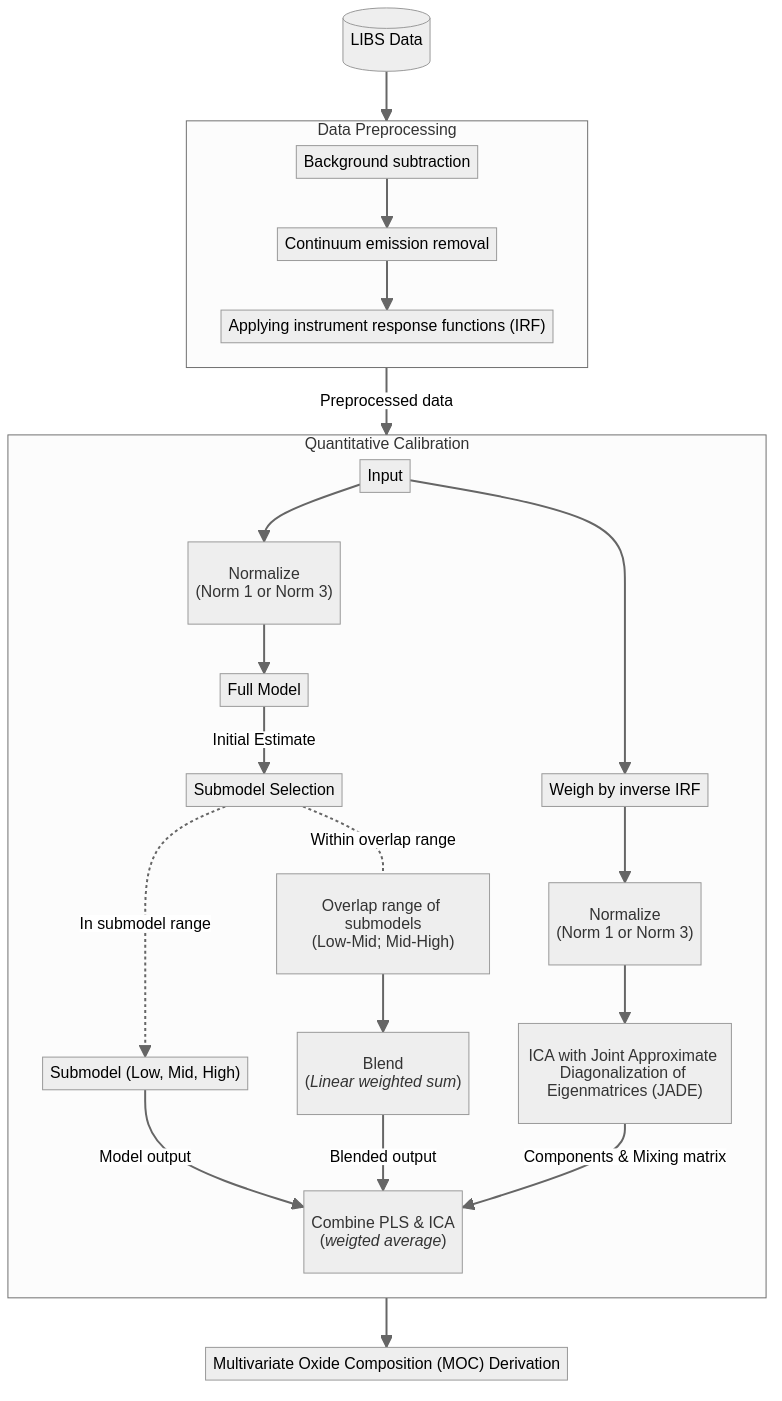
\includegraphics[width=0.225\textwidth]{images/pipeline.png}
    \caption{High level overview of the pipeline for deriving the MOC from raw LIBS data.}
    \label{fig:libs_data_processing}
\end{figure}

In Figure~\ref{fig:libs_data_processing} we illustrate the inference steps for deriving the MOC from LIBS data.
In Section~\ref{sec:methodology}, we detail the training process of the models.
A comprehensive description of the MOC model is presented in \citet{cleggRecalibrationMarsScience2017} and \citet{andersonImprovedAccuracyQuantitative2017}.
Here, we offer a concise summary of the MOC model, laying the groundwork for further exploration of our contributions to the subject.

\subsubsection{Data Preprocessing}\label{sec:data_preprocessing}
Before the MOC model can be applied to the data, the raw LIBS data must be preprocessed to produce a clean calibrated spectrum (CCS).
We do not go into further details about this process here, however a full description can be found in \citet{wiensPreFlight3}.
We only concern ourselves with the CCS data in this work.

The CCS data format is a table of intensity values for each wavelength, with each row representing the intensities for a given shot, which is a single laser pulse on the sample.
We give a more detailed description of the CCS data format in Section \ref{sec:data_overview} where we also describe the ChemCam calibration dataset as a whole.

\subsubsection{Multivariate Oxide Composition Derivation}\label{sec:moc_derivation}
The multivariate analysis adopts a hybrid methodology, blending Partial Least Squares Regression with Sub-models (PLS1-SM) and ICA to calculate the MOC.
The outcomes of these two techniques are merged using a weighted average for each oxide, with the weighting skewed in favor of the technique that demonstrates superior performance for the specific oxide.
The PLS1-SM approach utilizes tailored sub-models that specialize in targeting distinct composition ranges, along with a comprehensive full model used for initial composition estimation.
ICA assists in distinguishing elemental emission lines, contributing to a refined multivariate model.

Two normalization methods are employed in the analysis: Norm 1 and Norm 3.
Norm 1 standardizes the full spectrum across all three spectrometers such that the sum total is unity.
In contrast, Norm 3 conducts normalization on a per-spectrometer basis, culminating in a full normalized spectrum summing to three.
The optimal normalization technique is selected based on its efficacy in model performance for the specific analysis task at hand.

\subsubsection{Outlier Removal}\label{sec:outlier_removal}

In their analysis, \citet{andersonImprovedAccuracyQuantitative2017} employed a methodical outlier removal process to enhance model accuracy in multivariate regression. To detect outliers, they utilized influence plots, employing statistical measures that reflect each data point's deviation from the model's predictions and their influence on the model due to their position in the predictor space.
In this context, the deviation, or the error, are known as residuals and the influence a data point has on the model is known as leverage.
The application of the following equation to latent variables enables the computation of an observation's leverage vector (\(h_t\)):

\begin{equation}
    h_t = \text{diag}\left[ t(t^T t)^{-1} t^T \right],
\end{equation}

where $t$ represents the PLS scores.
Given that leverage quantifies the distance of each observation from the model's center, it can be interpreted as the square Mahalanobis distance --- a measure of the distance of a point from the center of mass of points in multivariate space.
If the original data follows a multivariate normal distribution, the distances form a chi-squared distribution. Using this property, outliers can be detected using the chi-square test \cite{brereton_chi_2015}.
The Mahalanobis distance is defined as follows:

\begin{equation}
    D_M(p)^2 = (p - \mu)^T \cdot \Sigma^{-1} (p - \mu),
\end{equation}

where $p$ is the point in question, $\mu$ is the mean of the distribution and $\Sigma^{-1}$ is the inverse of the covariance matrix of the distribution, known as the precision matrix.
Variables exhibiting a high leverage score are indicative of predictors that deviate more significantly from the others, thereby having a greater influence on the model.
The measure of model fit, denoted $Q$, is calculated by squaring the differences between the actual spectrum $x$ and the spectrum predicted by the model. This prediction uses the model's scores $t$ and loadings ($P$) to calculate the residuals $e$:

\begin{equation}
    e = x - t \cdot P^T.
\end{equation}

The fit of model for the $i$th observation is then computed by taking the residual vector $e_i$ and multiplying it by the transpose of itself $e^T$, which gives you the sum of squared differences\cite{marini_chemometrics_2013, andersonImprovedAccuracyQuantitative2017}:

\begin{equation}
    Q_i = e_{i}e_{i}^T.
\end{equation} 

Outlier removal is performed iteratively; an initial PLS model is conceived with cross-validation to determine the optimum number of latent variables, followed by an inspection of the influence plot to pinpoint outliers. Identified outliers are removed, and the model is re-evaluated. This procedure is repeated as needed, ensuring that any removals do not degrade the model's general performance.


\subsubsection{Partial Least Squares Sub-Models}\label{sec:pls_sub-models}

\citet{andersonImprovedAccuracyQuantitative2017} proposed an approach referred to as PLS1-SM.
The inherent variability in the responses of LIBS spectrometers to different concentrations of elements necessitates a nuanced analysis.
    High element concentrations can lead to spectral signal obscuration, often due to phenomena like self-absorption in strong lines, while at lower concentrations, there is a risk of spectral lines disappearing.
A single regression model typically falls short in accounting for such variations, leading to compromises in predictive precision for specific samples.

They deployed multiple regression models, each tailored to subsets of the entire composition range, targeting "low," "mid," and "high" concentrations along with a comprehensive "full model." This led to the formation of 30 distinct models, with selected sub-model ranges that prioritize both a robust dataset and precise compositional response.

Each sub-model was subjected to training, cross-validation, and optimization phases, which included the iterative outlier removal strategy mentioned in Section~\ref{sec:outlier_removal}.
The full model's preliminary composition estimation of unknown targets dictates the choice of subsequent sub-model(s) for refined prediction.
If the full model's prediction falls within the "low", "mid", or "high" ranges, the corresponding sub-model is selected for the final prediction.
However, if a prediction falls within two ranges, the sub-models corresponding to the two ranges are blended to produce the final prediction.
For example, a prediction falling within the "low" and "mid" ranges would be calculated by blending the predictions from the "low" and "mid" sub-models as follows:

\begin{align*}
w_{\text{mid}} &= \frac{y_{\text{full}}-y_{\text{blend range, min}}}{y_{\text{blend range, max}} - y_{\text{blend range, min}}} \\
w_{\text{low}} &= 1 - w_{\text{mid}} \\
y_{\text{final}} &= w_{\text{low}}\cdot y_{\text{low}} + w_{\text{mid}}\cdot y_{\text{mid}}
\end{align*}

where,

\begin{itemize}
    \item $w_{\text{low}}$ is the weight applied to the lower of the two models,
    \item $w_{\text{mid}}$ is the weight applied to the higher of the two models,
    \item $y_{\text{low}}$ is the prediction from the lower of the two models, and
    \item $y_{\text{mid}}$ is the prediction from the higher of the two models.
\end{itemize}

This applies analogously for predictions in the "mid-high" range to prevent prediction discontinuities.

The exact delineations of the blending ranges are adjustable, with optimization performed using the Broyden-Fletcher-Goldfarb\\-Shannon (BFGS) algorithm. This process, aimed at minimizing the RMSE for the full model dataset, established optimal ranges. Initial blend boundaries were predicated on sub-model intersections, with exceptional outliers managed distinctly due to their deviation from expected value ranges.

\subsubsection{Independent Component Analysis}\label{sec:ica}
\citet{cleggRecalibrationMarsScience2017} and \citet{forniIndependentComponentAnalysis2013} proposed the use of ICA to identify the elemental emission lines in LIBS spectra. ICA is a computational method used to separate a multivariate signal into additive, statistically independent components, particularly useful in scenarios where the signal sources overlap, such as in LIBS data.

ICA identifies independent components within the observed spectral data and produces a mixing matrix.
This matrix illustrates the combination of these independent components to reconstruct the original multivariate signal.

After extracting the independent components, the key task is to associate each independent component with a specific elemental emission line.
This process involves examining the emission lines of the elements and evaluating the ICA scores.
These scores reflect the correlation between each Independent Component and the entire spectrum of wavelengths.
Subsequently, these correlation values, sometimes referred to as ICA scores, are employed to establish a calibration curve, which correlates the ICA scores to the elemental compositions.

To ascertain the accuracy of this calibration, a regression analysis is performed using multiple regression functions. The function that provides the most reliable fit is used to predict the composition for each element.
